%!TEX root = ../dissertation.tex
\chapter{Problem Description} \label{cha:problem_description}

The problem addressed in this project is based on the classic blocks world problem\footnotemark{}. 
\footnotetext{\url{https://en.wikipedia.org/wiki/Blocks_world\#:~:text=In\%20its\%20basic\%20form\%2C\%20the,different\%20sizes\%2C\%20shapes\%20and\%20colors.}}
The blocks world is a planning domain in artificial intelligence and is used as a toy problem. From an algorithm perspective, it is an NP-Hard search and planning problem.
Here, a more general version of it is presented. \\
First of all, the environment consists of:
\begin{itemize}
	\item A robot manipulator, equipped with a video camera
	\item Blocks (cubes) in the same size, which all have an AprilTag \cite{olson2011tags, wang2016iros} attached to one of the faces
	\item Zero or more fixed objects, also with AprilTags
\end{itemize}

\begin{figure} [h]
\centering
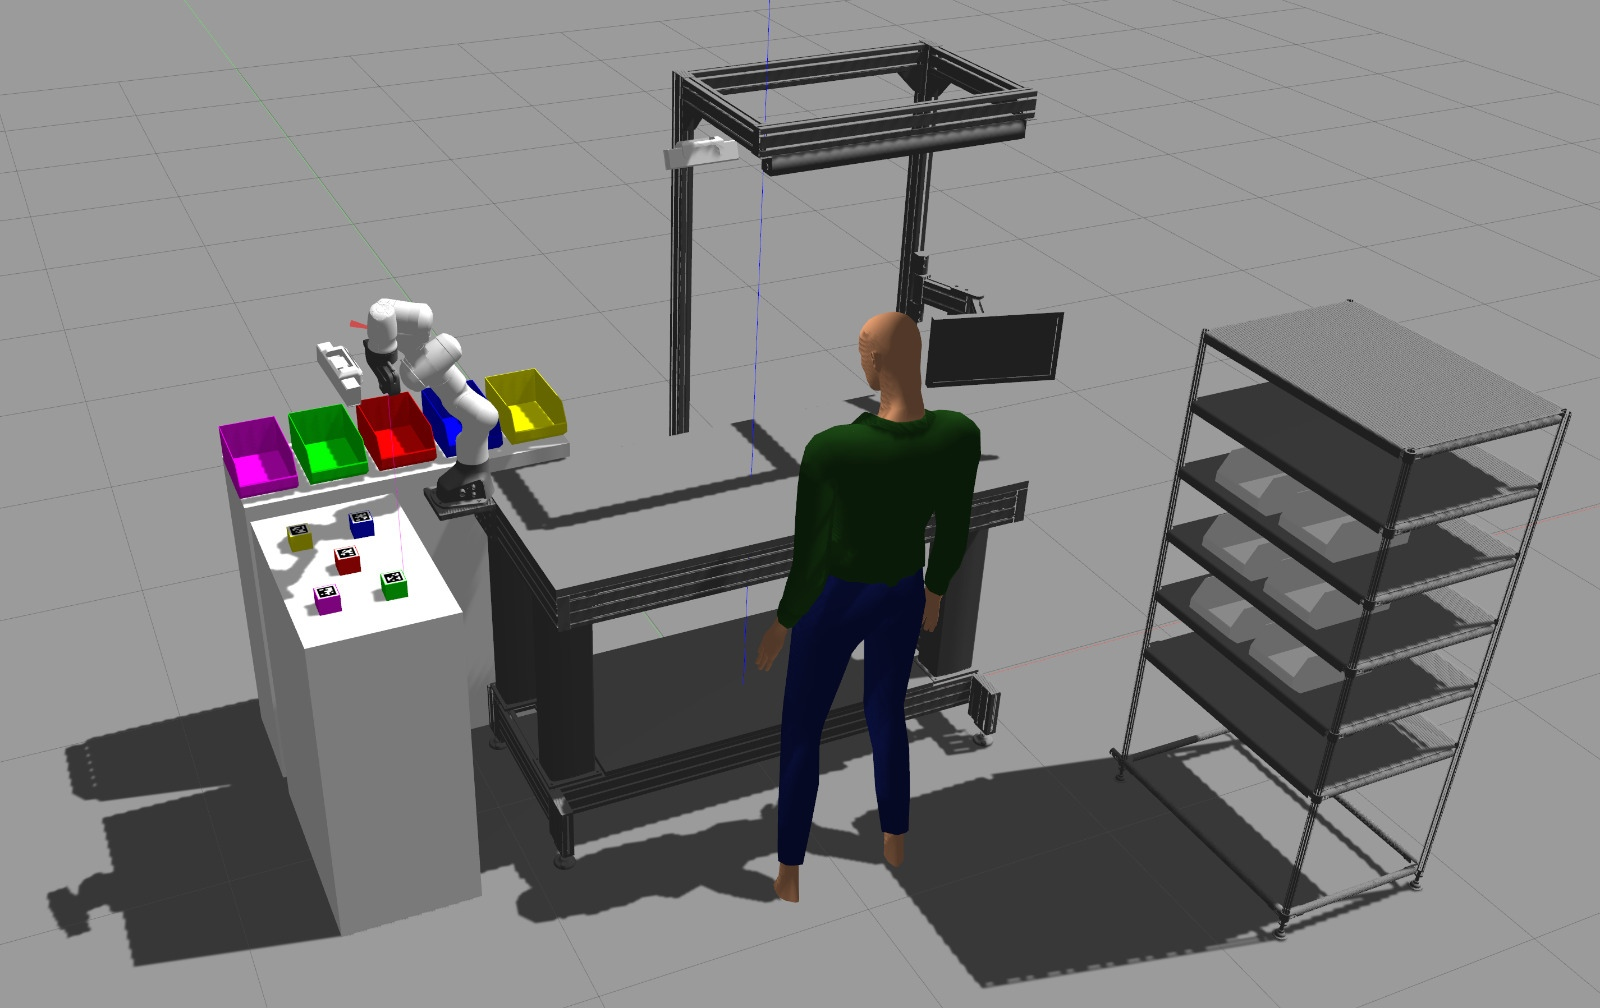
\includegraphics[width=0.9
\textwidth]{figures/Magistrale/env_1_temp}
\caption[Environment Configuration]{ IMMAGINE DA SISTEMARE
\label{fig:env_1}}
\end{figure} 

Figure \ref{fig:env_1} illustrates a possible configuration of the environment, which is the one used in this project. \\
Compared to the state-of-the-art, where the robot arm has to pick and place the blocks and the goal is to build one or more vertical stacks of them, the goal is generalized in a way that any arrangement of the blocks can be achieved. 
That is, given any initial arrangement of the blocks in the environment, find the shortest sequence of actions that the robot has to perform in order to achieve the required arrangement. \\

In order to define the implementation, it is first necessary to explain the constraints of this problem:

\begin{itemize}
	\item The robot knows only four actions: \textit{Pickup}, \textit{Putdown}, \textit{Stack}, \textit{Unstack}.
	\item Each block is \textit{clear} if and only if it has no object on it and is not \textit{in-hand} (i.e., the robot's hand can take it with a single action).
	\item Each block can be \textit{on} the table, on top of another object or \textit{in-hand}
	\item The robot's hand may be busy (it is holding a block) or free (it holds nothing)
	\item Only one block can be picked up at a time, putting it down before the next. It is not possible to pick up a block that is under another one (because it is not considered \textit{clear}) or to move a fixed object.
%% Aggiungi o rimuovi
\end{itemize}

The \textit{Pickup} action is the opposite of \textit{Putdown} and they are used to take/place a block from/on a fixed object. The \textit{Stack} action is the opposite of \textit{Unstack} and they are used to put/take a block on/from another block or a fixed object. \\
Basically these actions mirror physics. \\
For example, consider two blocks (A and B) on a table and block A is \textit{on} block B: to pick up block B, that block must be \textit{clear} and the hand must be free. Initially, block A is \textit{clear}, while B is not. Thus, one can do \textit{Unstack} of blocks A and B, getting block B \textit{clear} and block A \textit{in-hand}, then do \textit{Putdown} of block A and finally do \textit{Pickup} of block B, achieving the goal. Figure \ref{fig:blocks_example} illustrates these steps. \\

\begin{figure} [h]
\centering
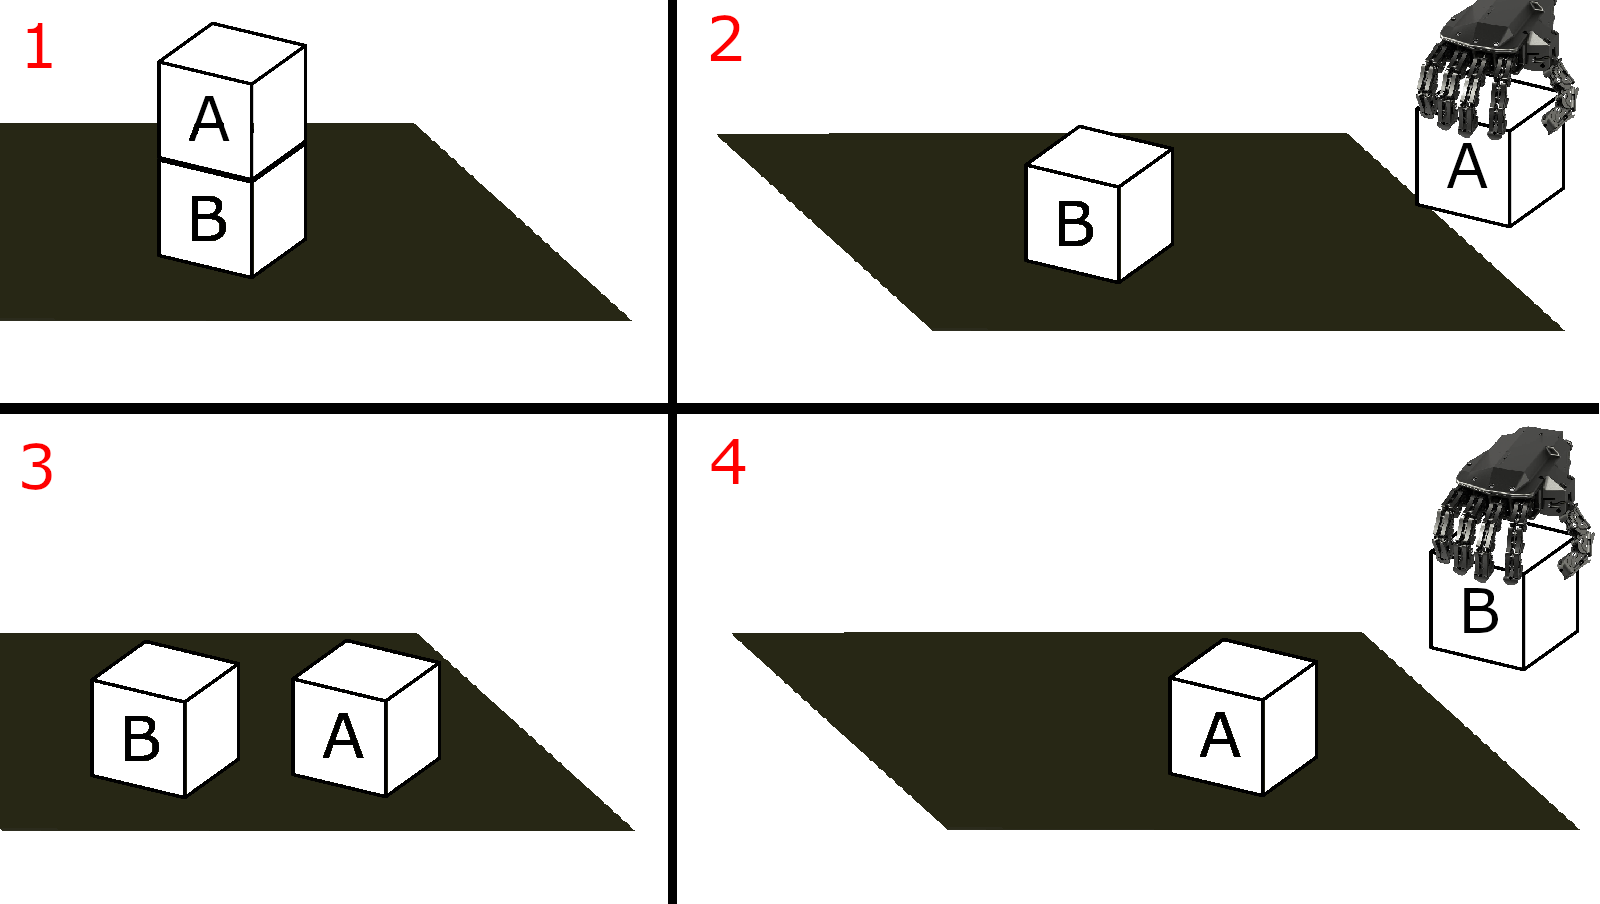
\includegraphics[width=0.9
\textwidth]{figures/Magistrale/blocks_example}
\caption[Blocks world example]{Three actions to go from state 1 (initial arrangement) to state 4 (target arrangement): \textit{Unstack} of A and B, \textit{Putdown} of A, \textit{Pickup} of B. 
\label{fig:blocks_example}}
\end{figure} 

Since it is possible to have more fixed objects (such as tables, shelves, etc.) than in the blocks world, where there is only a work plane, any free block can always be considered on top of something else. Consequently, the actions \textit{Pickup} and \textit{Putdown} lose their meaning because they become subcases of the respective \textit{Unstack} and \textit{Stack}. However, in this project all four are still maintained and used, as explained below. 


\section{Knowledge Base in Atomese}\label{sec:env_atomese}

Any aspect of the environment, the problem, the robot or anything else can be represented in the form of Atoms, which will populate the AtomSpace (i.e. the hypergraph of the KB). \\
There are many different ways of encoding these aspects. The one used in this project is proposed below. \\

Firstly, the Atomese representation of the objects: \\
\begin{python}
	(InheritanceLink
		(ConceptNode "apple")
		(ConceptNode "object"))

	(InheritanceLink
		(ConceptNode "table")
		(ConceptNode "fixed-object"))
\end{python}
On a practical (physical) level, the objects will all be cubes, except for the fixed ones. At the conceptual level, a semantic meaning will be associated to the AprilTags of each cube. In this way, and thanks to the AprilTags, it is possible to simplify the perception and manipulation of objects by replacing each different object with a cube. \\
In other words, it will be possible to \enquote{simulate} working with any kind of object, and thus demonstrate the potential of the NLP aspect of this project, leaving out perception and manipulation, which do not concern it at the moment. \\
For this reason, the code above speaks of \textit{apple} and not \textit{cube\_1}. \\

In that code, the \textit{apple} has been defined as an \textit{object} and the \textit{table} as a \textit{fixed-object}. 
ConceptNodes were used to refer to \enquote{concepts} and InheritanceLinks to connect two ConceptNodes with an \enquote{inheritance} meaning. This way, when the robot searches for which objects it can move, it will limit the pattern matching only to Atoms that are objects (thus, only to the apple). \\
As each atom is unique, it is not necessary to first define objects (i.e., \textit{apple} and \textit{table}) and concepts (i.e., \textit{object} and \textit{fixed-object}) and then, link them. Within the same AtomSpace, once an Atom is defined, whether independently or within any hypergraph, it will remain unique and the creation of other hypergraphs containing that Atom will not create a new one, but rather it will be shared between the various hypergraphs, in a sense, connecting them. \\

In addition, by construction of pattern matching rules, it is necessary to explicitly define the \enquote{non-equality} between all the various pairs of objects. Therefore, for example, given three objects such as \textit{apple}, \textit{tray} and \textit{table}, there will be Atoms like these: \\
\begin{python}
	(NotLink (EqualLink 
		(ConceptNode "apple") (ConceptNode "tray")))

	(NotLink (EqualLink 
		(ConceptNode "apple") (ConceptNode "table")))

	(NotLink (EqualLink 
		(ConceptNode "tray") (ConceptNode "table")))
\end{python}
They correspond to all possible simple combinations (without repetition) that can be constructed from the set of all objects (fixed ones included) taken two at a time. \\

Finally, now that the objects have been constructed, inherited and differentiated, one or more states must be associated with them. The best way to represent the state of an object is via an EvaluationLink, which associates a PredicateNode with one or more objects (their relative Atoms). The possible states of an object are: \textit{clear}, \textit{in-hand}, \textit{on}. Thus, for example: \\
\begin{python}
	(EvaluationLink
		(PredicateNode "clear")
		(ConceptNode "tray"))
	
	(EvaluationLink
		(PredicateNode "in-hand")
		(ConceptNode "apple"))
	
	(EvaluationLink
		(PredicateNode "on")
		(ListLink
			(ConceptNode "tray")
			(ConceptNode "table")))
\end{python}

In Appendix A, Section \ref{sec:KB_examples}, complete examples have been added.


\section{Actions in Atomese}\label{sec:domain_atomese}


Automated planning and scheduling problems, such as this one, are usually described in the notation Planning Domain Definition Language (PDDL), which is an AI planning language for symbolic manipulation tasks. In Appendix A, Section \ref{sec:PDDL} provides the domain and problem in PDDL format of the block world. 